\documentclass{beamer}
\usepackage{amsfonts,amsmath,oldgerm}
\usepackage[nameinlink]{cleveref}
\usepackage{graphicx}
\usepackage{hyperref}
\usepackage[
  backend=biber,
  style=alphabetic,
  sorting=anyt,
  minnames=3,
  minalphanames=3
]{biblatex}

\hypersetup{
    colorlinks=true,
    citecolor=red,
    linkcolor=white,
    urlcolor=black,
    pdftitle={MLCS Seminar},
}

\usetheme{sintef}

\newcommand{\N}{\mathbb{N}}
\renewcommand{\P}{\mathbb{P}}
\newcommand{\Z}{\mathbb{Z}}
\newcommand{\Q}{\mathbb{Q}}
\newcommand{\R}{\mathbb{R}}
\newcommand{\F}{\mathbb{F}}
\newcommand{\im}{\mathrm{im}}
\newcommand{\abs}[1]{\left|#1\right|}
\newcommand{\floor}[1]{\left \lfloor #1 \right \rfloor}
\newcommand{\abk}[1]{\left\langle#1\right\rangle}
\newcommand{\rbk}[1]{\left ( #1 \right )}
\newcommand{\ceil}[1]{\left \lceil #1 \right \rceil}
\newcommand{\curlyquotes}[1]{\textquotedblleft #1\textquotedblright}

\usefonttheme[onlymath]{serif}
\setbeamercovered{transparent}

\titlebackground*{assets/background}

\title{Degrees of Uncomputability: \\Post's problem and the Finite \\Injury Priority method}
% \subtitle{Mathematical Logic for Computer Science}
\course{Master's Degree in Computer Science}
\author{\href{https://github.com/Exyss/}{Simone Bianco}}
\IDnumber{1986936}
\date{Academic Year 2024/2025}

\addbibresource{../references.bib}

\begin{document}
\maketitle


% \begin{frame}

% This template is a based on \hrefcol{https://www.overleaf.com/latex/templates/sintef-presentation/jhbhdffczpnx}{SINTEF Presentation} from \hrefcol{mailto:federico.zenith@sintef.no}{Federico Zenith} and its derivation \hrefcol{https://github.com/TOB-KNPOB/Beamer-LaTeX-Themes}{Beamer-LaTeX-Themes} from Liu Qilong

% \vspace{\baselineskip}

% In the following you find a brief introduction on how to use \LaTeX\ and the beamer package to prepare slides, based on the one written by \hrefcol{mailto:federico.zenith@sintef.no}{Federico Zenith} for \hrefcol{https://www.overleaf.com/latex/templates/sintef-presentation/jhbhdffczpnx}{SINTEF Presentation}

% % This template is released under \hrefcol{https://creativecommons.org/licenses/by-nc/4.0/legalcode}{Creative Commons CC BY 4.0} license

% \end{frame}

\section{Introduction}

\begin{frame}{What is computation?}
\framesubtitle{Defining computation}

    \uncover<+->{
        1931 -- Kurt Gödel defines \textbf{General Recursive Functions} to prove his Incompleteness Theorems. It's the first mathematical definition of computation.
    }
    \uncover<+->{
        \begin{itemize}[<+->]
        \item \textit{Constant functions}: return the natural number $n$
        
        \item \textit{Successor function}: on input $x$ return $x+1$ 
        
        \item \textit{Projection function}: on input $(x_1, \ldots, x_n)$ return $x_i$ 
        
        \item \textit{Composition operator}: on input $h,g_1, \ldots, g_m$ return the function that applies $h$ together on the outputs of the applications of $g_1, \ldots, g_m$
        
        \item \textit{Primitive recursion operator}: on input $h,g$, return the function that applies $g$ if the first input is 0 and otherwise applies $h$ on the first argument $x_0$ and then recursively applies the process on the predecessor of $x$.
        
        \item \textit{Minimization operator}: on input $f$, search the first value $z$ that makes $f$ return 0 when $z$ is the first argument.
        \end{itemize}
    }
\end{frame}


\begin{frame}{What is computation?}
\framesubtitle{Defining computation}

    1931 -- Kurt Gödel defines \textbf{General Recursive Functions} to prove his Incompleteness Theorems.
    
    \begin{itemize}
    \item \textit{Constant functions}: $C_n^k(x_1, \ldots, x_k) := n$ for all $k,n \in \N$
    \item \textit{Successor function}: $S(x) := x+1$
    \item \textit{Projection function}: $P^k_i(x_1, \ldots, x_k) := x_i$ for all $k \in \N$
    \item \textit{Composition operator}: $(h \circ (g_1, \ldots, g_m))(x_1, \ldots, x_k) := h(g_1(x_1, \ldots, x_k), \ldots, g_m(x_1, \ldots, x_k))$
    \item \textit{Primitive recursion operator}: $\rho(g,h) := f$ where:
    \[f(x_0, x_1, \ldots, x_k) = \left \{ \begin{array}{ll}
        g(x_1, \ldots, x_k) & \text{if } x_0 = 0 \\
        h(y_0, f(y_0, x_1 \ldots, x_k)) & \text{if } x_0 = S(y_0) \\
    \end{array}\right .\]

    \item \textit{Minimization operator}: $\mu(f) := f'$ where:
    \[f'(x_1, \ldots, x_k) = \left \{ \begin{array}{ll}
        z & \text{if $f(z, x_1, \ldots, x_k) > 0$ and $f(i, x_1, \ldots, x_k) > 0$  for all $i <  z$}  \\
        * & \text{otherwise}
    \end{array}\right .\]
    \end{itemize}
\end{frame}

\begin{frame}{What is computation?}
\framesubtitle{Defining computation}

    1935 -- Alonzo Church defines \textbf{$\lambda$-calculus} to settle the Entscheidungsproblem problem.
    
    \begin{itemize}[<+->]
        \item \textit{Language grammar}: $M,N ::= x \mid \lambda x.M \mid MN$
        \item \textit{Substitution}: $M[x := N]$ means that $x$ gets substituted by $N$ in $M$
        \item \textit{$\alpha$-rule}: $\lambda x.M \xrightarrow{\alpha} \lambda y.(M[x := y])$
        \item \textit{$\beta$-rule}: $(\lambda x.M)N \xrightarrow{\beta} M[x := N]$
        \item \textit{$\eta$-rule}: $\lambda x. Mx \xrightarrow{\eta} M$ if $x \notin \mathrm{free}(M)$
    \end{itemize}

    \quad

    \uncover<+->{
        Stephen Kleene proves that $\lambda$-calculus is equivalent to general recursive functions
    }
\end{frame}

\begin{frame}{What is computation?}
\framesubtitle{Defining computation}

    1936 -- Alan Turing defines a simple abstract model of a computer.

    \begin{itemize}[<+->]
        \item Infinite tape subdivided in cells with a read-write head
        \item Set of instructions defined by a function $\delta$
        \item Each instruction moves the head left or right based on the current state and the value read.
        \item It may also change the value below the head before moving.
    \end{itemize}

    \quad

    \uncover<+->{
        Turing's machine also settles the Entscheidungsproblem and it is equivalent to $\lambda$-calculus.

        Recognized by Gödel himself as the best definition of computation.
    }
\end{frame}

\begin{frame}{What is computation?}
\framesubtitle{Defining computation}

    $\Phi_{i,s}(x)$ denotes the \textbf{computation} of the $i$-th TM for $s \in \N$ steps on input $x \in \N$.

    \uncover<+->{
        \begin{itemize}[<+->]
        \item $\Phi_{i,s}(x) \downarrow$ : the computation halts after $s$ steps
        \item $\Phi_{i}(x) \downarrow$ : there is a $s \in \N$ such that $\Phi_{i,s}(x) \downarrow$
        \item $\Phi_{i}(x) \uparrow$ : there is no $s \in \N$ such that $\Phi_{i,s}(x) \downarrow$
        \item $\psi_{i}(x)$ : output of the computation (defined iff $\Phi_{i}(x) \downarrow$)
        \end{itemize}
    }
\end{frame}

\begin{frame}{Computability}
\framesubtitle{Definitions}

    Given a set $S \subseteq \N$, we say that $S$ is:
    \begin{itemize}[<+->]
        \item \textbf{Semi-decidable} when $\exists i \in \N$ such that $\forall x \in \N$ it holds that $\psi_i(x) = 1$ if $x \in S$, otherwise $\psi_i(x) = 0$ or $\Phi_i(x) \uparrow$.
        \item \textbf{Decidable} when $\exists i \in \N$ such that $\forall x \in \N$ it holds that $\psi_i(x) = 1$ if $x \in S$, otherwise $\psi_i(x) = 0$.
        \item \textbf{Recursively enumerable} when there is an algorithmic procedure $\mathcal{A} : \N \to \{0,1\}$ such that $S = \{A(0), A(1), A(2), \ldots\}$
    \end{itemize}

    \quad

    \uncover<+-> {
        \textbf{Obs. 1:} $S$ is semi-decidable if and only if it is recursively enumerable

        \textbf{Obs. 2:} $S$ is decidable if and only if both $S$ and $\overline{S}$ are semi-decidable.
    }
\end{frame}

\begin{frame}{Introduction}
\framesubtitle{Turing's work}
    \textcite{turing} proved that:
    \begin{itemize}[<+->]
        \item  Some sets that are semi-decidable but undecidable (e.g. $H = \{\abk{i,x} \mid \Phi_i(x) \downarrow\}$).
        
        \item Some sets cannot be semi-decided (e.g. $\overline{H}$).
    \end{itemize}

    \quad

    \uncover<+-> {
        Three degrees of computability: \textbf{solvable} problems, \textbf{semi-solvable} problems and \textbf{unsolvable} problems.

        \quad

        Are there some other degrees of computability?
    }
\end{frame}

\section{Degrees of uncomputability}

\begin{frame}{Degrees of uncomputability}
\framesubtitle{Turing degrees}
    \textcite{post_degrees} formalized the idea of computability degrees through \textbf{Turing reductions}.

    \quad

    \uncover<+->{
        Let $\Phi_i^B$ denote the Turing machine $\Phi_i$ with access to an oracle machine that decides $B$.
    }

    \begin{itemize}[<+->]
        \item \textit{Turing reducibility}: $A \leq_T B$ when $\exists i \in \N$ such that $\Phi_i^B(x) \downarrow$ for all $x \in \N$ and $A = \{x \in \N \mid \psi_i^B(x) = 1\}$.
        
        \item \textit{Turing equivalence}: $A \equiv_T B$ when $A \leq_T B$ and $B \leq_T A$
        
        \item The set $\mathcal{D} = 2^{\N}/_{\equiv_T}$ is the set of \textbf{Turing degrees}.
        \item $[A]$ is the class containing $A$ over $\mathcal{D}$.
    \end{itemize}
\end{frame}

\begin{frame}{Degrees of uncomputability}
\framesubtitle{Turing degrees}

    \begin{itemize}[<+->]
        \setlength{\itemindent}{-2em}

        \item[] We say that $[A]$ is \textbf{lower} than $[B]$, written as $[A] \preceq [B]$, if $A \leq_T B$.
        
        \quad
        
        \item[] $\preceq$ forms an ordering over the set $\mathcal{D}$, giving an hierarchy of unsolvability degrees.
        
        \quad
        
        \item[] $0 = [\varnothing]$ is the unique degree containing all decidable problems
        \begin{itemize}
            \item There is no degree below $0$
            \item $0$ is lower than any degree
        \end{itemize}
    \end{itemize}
\end{frame}

\begin{frame}{Degrees of uncomputability}
\framesubtitle{The jump operator}
    The strict relation $[A] \prec [B]$ between degrees can be easily forced through \textbf{Turing jumps}.
    \begin{itemize}[<+->]
        \item Given a set $X \subseteq \N$, the \textit{Turing jump} of $X$ is the set $X' = \{\abk{i,x} \mid \Phi_i^X(x) \downarrow\}$
        \begin{itemize}
            \item $X \leq_T X'$ but $X' \not\leq_T X$ since $X'$ is a variant of the Halting problem using $X$ as an oracle.
        \end{itemize}

        \quad

        \item The jump of $\varnothing$ is exactly the Halting problem $H$
        \item We define $0'$ as the class of $H$ (or $\varnothing'$)
    \end{itemize}
\end{frame}

\begin{frame}{Degrees of uncomputability}
\framesubtitle{Low degrees}
    \begin{itemize}[<+->]
        \item The jump operator can be iteratively applied to get infinite levels of the hierarchy
        \item A degree is said to be r.e. if it contains an r.e. set
        \item Not all sets inside an r.e. degree are r.e. (e.g. $\overline{H} \in 0'$)
        \item All r.e. degrees are below $0'$
        \begin{itemize}
            \item Equivalently, all degrees above $0'$ are not r.e.
        \end{itemize}
        \item Degrees below $0'$ are referred to as \textbf{low degrees}
    \end{itemize}
\end{frame}

\begin{frame}{Degrees of uncomputability}
\framesubtitle{Low degrees}

    \begin{figure}[H]
        \centering
        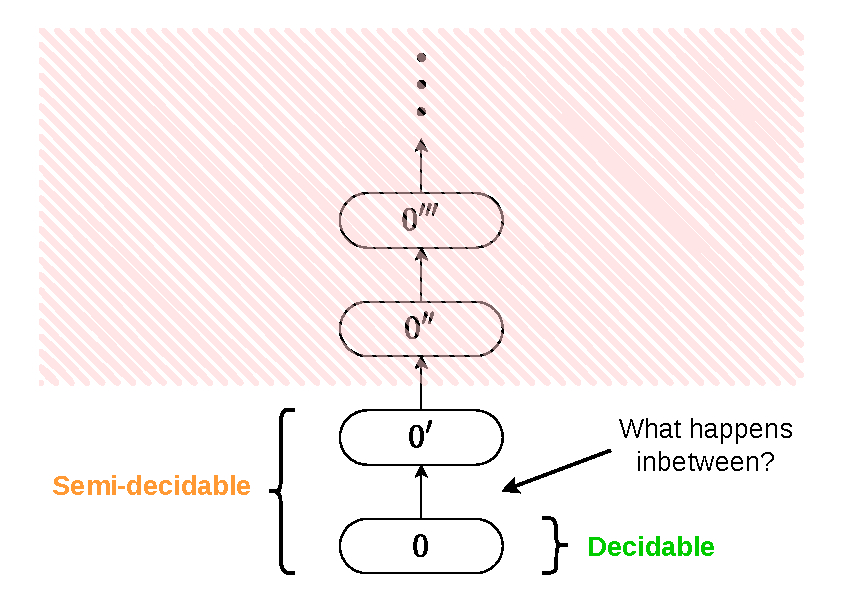
\includegraphics[scale=0.625]{../images/hierarchy_2.pdf}
    \end{figure}
\end{frame}


\begin{frame}{Degrees of uncomputability}
\framesubtitle{Post's problem}
    \begin{itemize}[<+->]
        \item In \cite{post_degrees}, Emil Post investigates the existence of a degree $d$ such that $0 \prec d \prec 0'$
        \item He was able to prove that for each degree $A \neq 0$ there is another degree $B$ that is incomparable with $A$.
        \begin{itemize}
            \item He was also able to force that $A$ and $B$ are low set
            \item This answers his original question
        \end{itemize}
        \item However, he couldn't find a way to force $A$ and $B$ to be r.e.
    \end{itemize}

    \quad

    \uncover<+->{
        \textbf{Post's problem}: is there a r.e. degree $d$ such that $0 \prec d \prec 0'$?
    }
\end{frame}

\section{The Finite Extension method}

\begin{frame}{The Finite Extension method}
\framesubtitle{Towards the solution to Post's problem}
    \begin{itemize}[<+->]
        \item Post's problem was solved 12 years later independently by \textcite{friedberg, muchnik} through the \textbf{finite injury priority method}.
        \item The method is an improvement on the \textbf{finite extension method} developed by Post in his original works
        \item Since the FIP method involves constructions that are way more complex than those of the FE method, we'll first give an example of the latter
    \end{itemize}
\end{frame}

\begin{frame}{The Finite Extension method}
\framesubtitle{The idea}

    \begin{itemize}[<+->]

        \item We define a list of requirements $\{R_i\}_{i \in \N}$ that will enforce our desired property over the sets $A$ and $B$
        
        \item We construct two list of strings$\{\alpha_i\}_{i \in \N}$ and $\{\beta_i\}_{i \in \N}$ where:
        \begin{itemize}
            \item $\alpha_i$ is a finite extension of $\alpha_{i-1}$ (same goes for $\beta_i$ and $\beta_{i-1}$)
            \item The strings $\alpha_i, \beta_i$ will satisfy requirement $R_i$
            \item Strings are to be considered as partial functions from $\N$ to $\{0,1\}$ (equivalently, as an infinite tape over $\{0,1,*\}$)
        \end{itemize}

        \item The sets $A = \bigcup_{i = 0}^{+\infty}\N[\alpha_i]$ and $B = \bigcup_{i = 0}^{+\infty}\N[\beta_i]$ will have our desired property
        \begin{itemize}
            \item $\N[s] = \{x \in \N \mid s(x) = 1\}$ is the set of all natural numbers \curlyquotes{selected} by $s$
        \end{itemize}
        
    \end{itemize}
\end{frame}

\begin{frame}{The Finite Extension method}
\framesubtitle{The Kleene-Post theorem}
    \cite{kleene_post} \textbf{Theorem:} There are two low sets $A$ and $B$ that are incomparable
    \begin{itemize}[<+->]
        \item Requirements:
        \[R_{2j} := (\psi_j^A \neq B) \qquad\qquad R_{2j+1} := (\psi_j^B \neq A)\]
        \item Start by setting $\alpha_0 = \beta_0 = \varepsilon$
    \end{itemize}
\end{frame}

\begin{frame}{The Finite Extension method}
\framesubtitle{The Kleene-Post theorem}
    \begin{itemize}[<+->]
        
        \item Consider any index $2j > 0$. Pick any position $x \in \N$ such that $\beta_{2j-1}(x) = *$ (guaranteed to exist)
        \item If there is any finite extension $\alpha'$ of $\alpha_{2j-1}$ such that $\Phi_{2j-1}^{\{\alpha'\}}(x) \downarrow$, we set:
        \[\alpha_{2j} = \alpha' \qquad \beta_{2j}(y) = \left \{ \begin{array}{ll}
            1-\psi_{2j}^{\{\alpha'\}}(x) & \text{if } y = x \\
            \beta_{2j-1}(y) & \text{otherwise}
        \end{array}\right .\]

        \item Otherwise, we set:
        \[\alpha_{2j} = \alpha_{2j-1} \qquad \beta_{2j}(y) = \left \{ \begin{array}{ll}
            \mathrm{rand}(\{0,1\}) & \text{if } y = x \\
            \beta_{2j-1}(y) & \text{otherwise}
        \end{array}\right .\]
    \end{itemize}
\end{frame}

\begin{frame}{The Finite Extension method}
\framesubtitle{The Kleene-Post theorem}
    
    \begin{figure}[H]
        \centering
        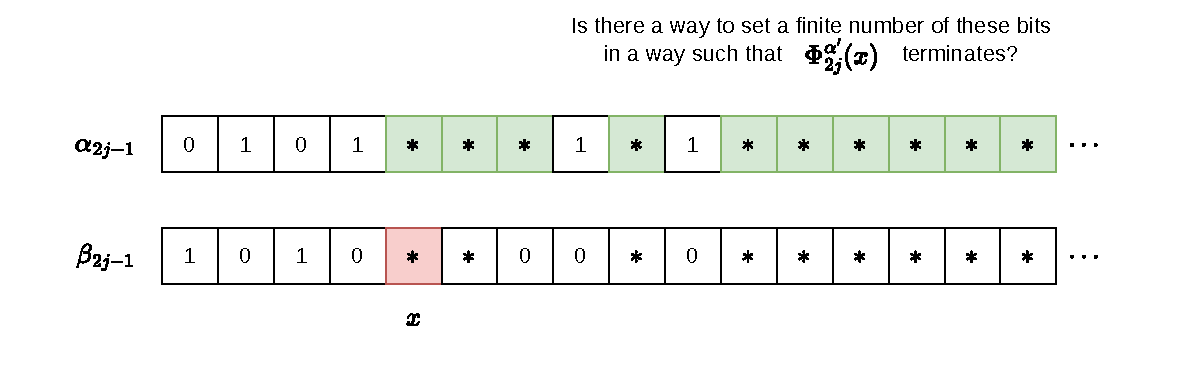
\includegraphics[scale=0.65]{../images/finite_extension_1.pdf}
    \end{figure}
\end{frame}

\begin{frame}{The Finite Extension method}
\framesubtitle{The Kleene-Post theorem}
    
    \begin{figure}[H]
        \centering
        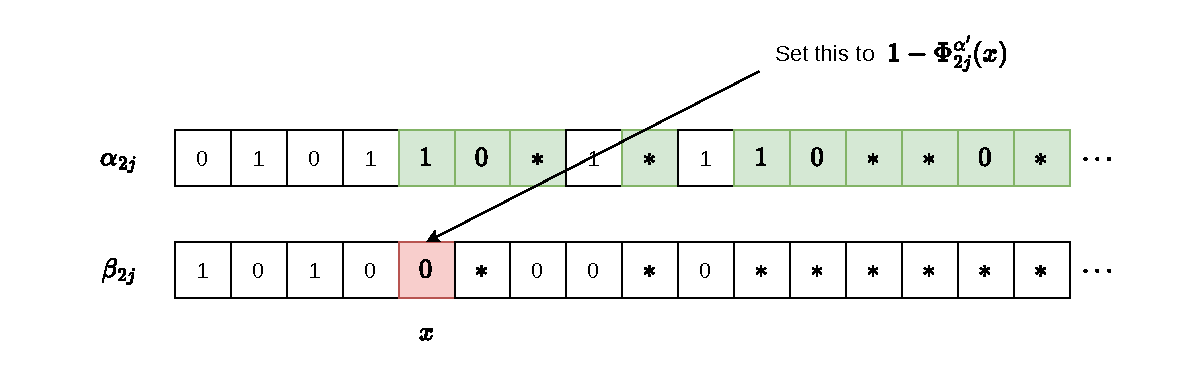
\includegraphics[scale=0.65]{../images/finite_extension_2.pdf}
    \end{figure}
\end{frame}

\begin{frame}{The Finite Extension method}
\framesubtitle{The Kleene-Post theorem}
    \begin{itemize}[<+->]
        \item Strings $\alpha_{2j}, \beta_{2j}$ satisfy requirement $R_{2j}$
        \item Symmetrical idea applied to index $2j+1 > 0$, satisfying $R_{2j+1}$
        \item \textbf{Incomparability}: all requirements are satisfied
        \item \textbf{Lowness}: $A$ and $B$ can be enumerated through an oracle for $H$ but \underline{not} without it
    \end{itemize}
    $\hfill \square$
\end{frame}

\begin{frame}{The Finite Extension method}
\framesubtitle{Strenghts and weaknesses}
    
    \begin{itemize}[<+->]
        \item We observe that this general method can be easily modified and extended.
        \item For instance, 
        \[R_{2j} := (\text{If } W_j \text{ infinite then }  W_j \cap A \neq \varnothing) \qquad\qquad R_{2j+1} := (\psi_j^B \neq A)\]
        imposes that $A$ is a \textbf{simple set} and that $B$ is a low set such that $A \not\leq_T B$
        \begin{itemize}
            \item $W_j = \{x \in \N \mid \Phi_j(x) \downarrow\}$
            \item $A$ is \textit{simple} when $A$ is r.e., $\overline{A}$ is infinite and $\overline{A}$ doesn't contain an infinite r.e. set
        \end{itemize}
    \end{itemize}
\end{frame}

\section{The Finite Injury Priority method}

\begin{frame}{The Finite Injury Priority method}
\framesubtitle{The idea}
    \begin{itemize}[<+->]
        \item \textbf{Injury}: a requirement gets injured when its satisfaction is not guaranteed anymore.
        
        \item The key idea is to assign a priority level to each requirement and force two conditions during the construction of the sets:
        \begin{enumerate}
            \item Each requirement has finitely many requirements with higher priority
            \item Each requirement can be injured only by requirements with higher priority
        \end{enumerate}

    \item We'll use \textit{sets} instead of strings to construct $A$ and $B$
    \end{itemize}

\end{frame}


\begin{frame}{The Finite Injury Priority method}
\framesubtitle{The query function}
    \begin{itemize}[<+->]
        \item To keep track of injuries, we'll use a \textbf{query function} $\omega_{i,s}^A(x)$ that returns the largest index queried by $\Phi_{i,s}^A(x)$.
        
        \[\omega_{i,s}^A(x) = \left \{ \begin{array}{ll}
            \max \{z \in \N \mid z \text{ gets queried in } \Phi_{i,s}^A(x)\} & \text{if } \Phi_{i,s}^A(x) \downarrow \\
            -1 & \text{otherwise}
        \end{array}\right .\]

        where $A  \subseteq \N$ and $i,s,x \in \N$.
    \end{itemize}

\end{frame}

\begin{frame}{The Finite Injury Priority method}
\framesubtitle{The Friedberg-Muchnik theorem}
    \cite{friedberg,muchnik} \textbf{Thm.:} There are two r.e. sets $A$ and $B$ that are incomparable
    \begin{itemize}[<+->]
        \item Requirements:
        \[R_{2j} := (\psi_j^A \neq B) \qquad\qquad R_{2j+1} := (\psi_j^B \neq A)\]
        \item Start by setting $A_0 = B_0 = \varnothing$
        \item We say that an index $x$ is a \textbf{witness} for the requirement $R_{2i}$ at step $s$ if $\Phi_{i,s}^{B_s}(x) \downarrow$ and $\psi_{i,s}^{B_s}(x) \neq A_s(x)$ (symmetric definition for $R_{2i+1}$)
    \end{itemize}
\end{frame}

\begin{frame}{The Finite Injury Priority method}
\framesubtitle{The Friedberg-Muchnik theorem}
    \begin{itemize}[<+->]
        \item On each step $s \in \N$, for each $j \in \N$ we compute:
        \begin{itemize}
            \item A witness $w_{j,s}$ for $R_j$ at step $s$
            \item A restriction index $r_{j,s}$ to fix the priority of the requirements
        \end{itemize}
        \item \textbf{Invariants}:
        \begin{itemize}
            \item $w_{j,s} = r_{j,s} = -1$ when no witness is known for $R_j$ at step $s$
            \item Indices that come before $r_{j,s}$ don't break any requirement.
        \end{itemize}
        \item $R_j$ gets \textit{injured} at step $s$ if $A_{s+1} - A_s$ contains some $x \leq r_{j,s}$.
    \end{itemize}
\end{frame}

\begin{frame}{The Finite Injury Priority method}
\framesubtitle{The Friedberg-Muchnik theorem}
    \begin{itemize}[<+->]
        \item Let $A_0 = B_0 = \varnothing$ and let $w_{j,0} = r_{j,0} = -1$ for each $j \in \N$.
        \item Consider a generic step $s = 2i$ (symmetrical argument for $s = 2i+1$).
        \item For each $j \leq s$, if $w_{j,s-1} \neq -1$ we propagate the previous values because $R_{2i}$ already has a witness.
        \begin{itemize}
            \item $A_{s} = A_{s-1}$ and $B_{s} = B_{s-1}$
            \item $w_{j,s} = w_{j,s-1}$ and $r_{j,s} = r_{j,s-1}$
        \end{itemize}
    \end{itemize}
\end{frame}

\begin{frame}{The Finite Injury Priority method}
\framesubtitle{The Friedberg-Muchnik theorem}
    \begin{itemize}[<+->]
        \item Suppose now that $w_{2h,s-1} = -1$.
        \item Let $x$ be the minimum index such that $x \notin A_{s-1}$ and such that for all $k < 2h$ it holds that $x > r_{k,s}$.
        \item If $\Phi_{h,s-1}^{B_{s-1}}(x) \uparrow$, we preserve that $w_{2h,s} = r_{2h,s} = -1$ and propagate $A_{s} = A_{s-1}$, $B_{s} = B_{s-1}$. This trivially satisfies the requirement $R_{2h}$.
        \item Otherwise, if $\psi_{h,s-1}^{B_{s-1}}(x) = 0$, we set:
        \[\begin{array}{ccc}
            w_{2h,s} = x & \qquad & r_{2h,s} = \max(x, \omega_{h,s-1}^{B_{s-1}}(x))\\\\
            A_{s} = A_{s-1} \cup \{x\} & \qquad & B_{s} = B_{s-1}
        \end{array}\]
    \end{itemize}
\end{frame}

\begin{frame}{The Finite Injury Priority method}
\framesubtitle{The Friedberg-Muchnik theorem}
    \begin{itemize}
        \item Suppose now that $w_{2h+1,s-1} = -1$.
        \item Let $x$ be the minimum index such that $x \notin B_{s-1}$ and such that for all $k < 2h+1$ it holds that $x > r_{k,s}$.
        \item If $\Phi_{h,s-1}^{A_{s-1}}(x) \uparrow$, we preserve that $w_{2h+1,s} = r_{2h+1,s} = -1$ and propagate $A_{s} = A_{s-1}$, $B_{s} = B_{s-1}$. This trivially satisfies the requirement $R_{2h+1}$.
        \item Otherwise, if $\psi_{h,s-1}^{A_{s-1}}(x) = 0$, we set:
        \[\begin{array}{ccc}
            w_{2h+1,s} = x & \qquad & r_{2h+1,s} = \max(x, \omega_{h,s-1}^{A_{s-1}}(x))\\\\
            A_{s} = A_{s-1} & \qquad & B_{s} = B_{s-1} \cup \{x\}
        \end{array}\]
    \end{itemize}
\end{frame}

\begin{frame}{The Finite Injury Priority method}
\framesubtitle{The Friedberg-Muchnik theorem}
    \begin{figure}
        \centering
        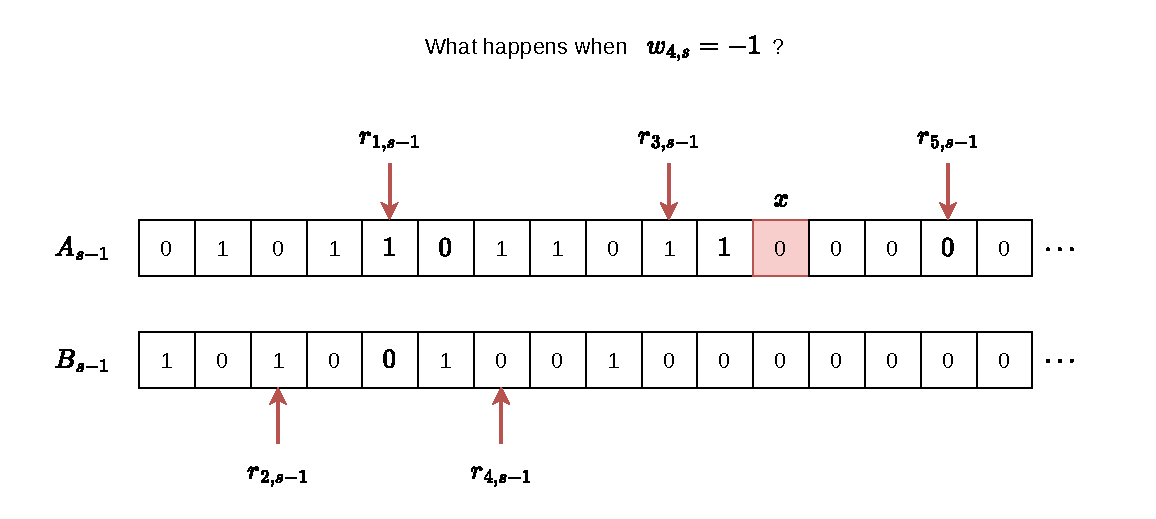
\includegraphics[scale=0.65]{../images/finite_injury_1.pdf}
    \end{figure}
\end{frame}

\begin{frame}{The Finite Injury Priority method}
\framesubtitle{The Friedberg-Muchnik theorem}
    \begin{figure}
        \centering
        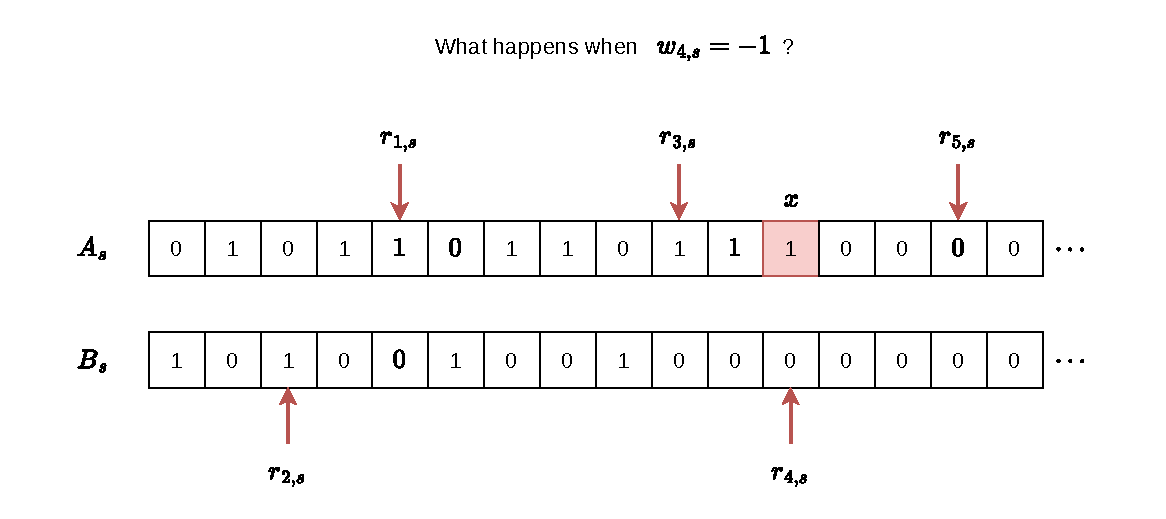
\includegraphics[scale=0.65]{../images/finite_injury_2.pdf}
    \end{figure}
\end{frame}

\begin{frame}{The Finite Injury Priority method}
\framesubtitle{The Friedberg-Muchnik theorem}
    \textbf{Claim}: For each $j \in \N$ it holds that:
    \begin{enumerate}
        \item $R_j$ is injured a finite number of times
        \item There is a step $s_0$ such that for all $s \geq s_0$ and for all $k < j$ no new index is added to $A_s$
    \end{enumerate}

    \textit{Proof.}
    \begin{itemize}[<+->]
        \item The requirement $R_j$ is injured at step $s$ if some $x \leq r_{j,s}$ is added to $A_{s-1}$ (or to $B_{s-1}$), which happens only when $w_{j,k} = -1$ and $\psi_{j,s}^{B_s}(x) = 0$ (or $\psi_{j,s}^{A_s}(x) = 0)$
        \item In other words, statement 2. of the claim follows from statement 1. by construction.
    \end{itemize}
\end{frame}

\begin{frame}{The Finite Injury Priority method}
\framesubtitle{The Friedberg-Muchnik theorem}
    \begin{itemize}[<+->]
        \item Let $g_{j,s} = \sum\limits_{\substack{k <\, j \; s.t. \\ w_{k,s} \neq -1}} 2^{-(k+1)}$ be the injure value of $R_j$ at step $s$
        \item When $R_j$ is injured at step $s-1$, the smallest value $k < j$ such that $w_{k,s-1} \neq w_{k,s}$ must satisfy $w_{k,s-1} = -1$ and $w_{k,s} \neq -1$ by construction. Thus:
        \[g_{j,s} - g_{j,s-1} \geq 2^{-(j+1)} - \sum_{k < h < j} 2^{-(h+1)} = 2^{-j}\]

        \item Hence, for each step $s$ we have that $0 \leq g_{j,s} \leq 1-2^{-j}$, concluding that $R_j$ can be injured at most $2^{j}-1$ times
    \end{itemize}
\end{frame}

\begin{frame}{The Finite Injury Priority method}
\framesubtitle{The Friedberg-Muchnik theorem}

    \begin{itemize}
        \item We observe that there is always a large enough step $s_0^*$ satisfying statements 1. and 2. of the Claim.
        
        \item This step guarantees that for each $j \in \N$ it holds that $\lim\limits_{s \to +\infty} w_{j,s}$ and $\lim\limits_{s \to +\infty} r_{j,s}$ exist and are finite.
        \begin{itemize}
            \item If for some $s' \geq s_0^*$ it holds that $w_{j,s'} \neq -1$ then it will hold from $s'$ onward
            \item Otherwise, there is a minimum value $x_s^*$ such that $x_s^* \notin A_s$ and such that $x_s^* > r_{k,s}$ for all $k < j$
            \item By construction $\Phi_{j,s}^{B_s}(x) \uparrow$ holds in this case
        \end{itemize}
    \end{itemize}

\end{frame}


\begin{frame}{The Finite Injury Priority method}
\framesubtitle{The Friedberg-Muchnik theorem}

    \begin{itemize}[<+->]
        \item $A = \bigcup_{s = 0}^{+\infty} A_s$ and $B = \bigcup_{s = 0}^{+\infty} B_s$ 
        \item The claim implies that every requirement will be, eventually, satisfied by the construction.
        \item Moreover, the use of the restriction values $r_{j,s}$ allows us to recursively enumerate the sets $A$ and $B$ by restricting our interest to the indexes between $0$ and $r_{j,s}$ for each $j \in \N$
        \begin{itemize}
            \item This implies that $A$ and $B$ are both r.e.!
        \end{itemize}
    \end{itemize}

    $\hfill \square$

\end{frame}

\begin{frame}{The Finite Injury Priority method}
\framesubtitle{Other interesting results}
    \begin{itemize}[<+->]
        \item \textbf{Infinite Injury Priority Argument}: \textcite{sacks} proved that the above construction can be extended to a countably infinite argument
        
        \item \textbf{Density of r.e. sets}: For each pair of r.e. sets $A, B$ there is another r.e. set $C$ such that $A <_T C <_T B$
        \item \textcite{simpson} proved that the first-order theory of $\mathcal{D}$ over the language $(\preceq, = )$ is many-one equivalent to the theory of true second-order arithmetic. 
    \end{itemize}
\end{frame}

\backmatter[notitle]
    
\begin{frame}{Bibliography}
\framesubtitle{{}}
    \printbibliography
\end{frame}

\end{document}
